\section{実験}
手法1について,通信確立の確認と,UDPでのP2P通信確立時との速度の比較を行った.手法2については他手法と比較を行う程度まで実装が及ばなかったため,前章で示したNAT越えで通信が確立したことを確認した

\subsection{実行環境}
両手法の実行について,片方のピアはMac OS 13.5 (Ventura),片方はGoogle CloudのCompute Engineを利用し,Ubuntu 18.0.4の仮想マシンを利用した.双方ともローカルネットワーク内に存在し,NATタイプはFull-Cone NATである.手法1で利用する仲介サーバーはHerokuにデプロイして実行した.

通信を確認するためのパケットキャプチャはWireshark 4.2.2を利用した.

\subsection{手法1の実験}
\subsubsection{通信確立の確認}
\begin{figure}[h]
  \centering
  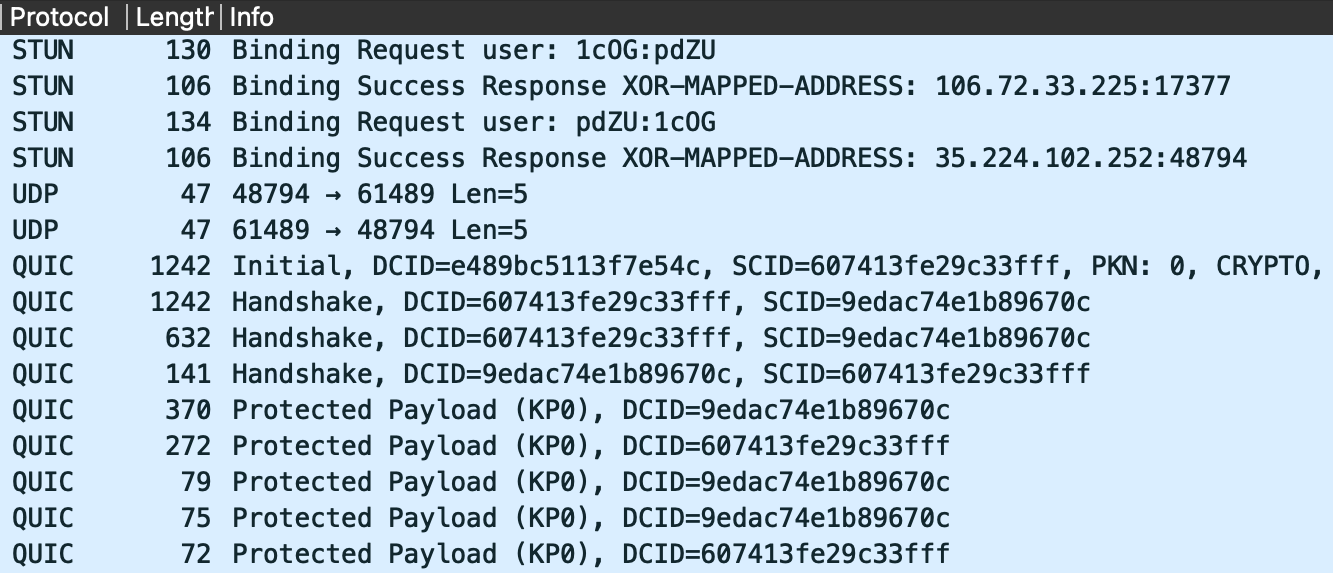
\includegraphics[width=\linewidth]{figs/ice-eva.png}
  \caption{手法1の実行結果}
  \label{fig:eva-1}
\end{figure}

手法1の通信確立が確認できた際のピア間のパケットキャプチャの様子を図~\ref{fig:eva-1}に示す.STUNパケットを用いた接続性チェックの後,QUICでのハンドシェイクが始まり,その後通信が確立されている.
\subsubsection{UDPでのP2P通信確立のみとの比較}
UDPでのP2P通信確立は単にICEプロトコルを用いて行った.手法1はICEプロトコルでの通信確立の後にQUICハンドシェイクを行っているため,UDPでの通信確立に比べて速度が遅くなることは自明である.

比較は,手法1を30回実行し,ICEプロトコルの通信が確立するまでの秒数,その後のQUICハンドシェイクまで含めた秒数をそれぞれ計測し平均を算出した.

ICEプロトコルの通信が確立するまでは平均で約4.82秒,その後のQUICハンドシェイクまで含めると約5.35秒であった.つまりQUICのハンドシェイクには約0.5秒かかっていることになる.

\subsection{手法2の実験}
\begin{figure}[h]
  \centering
  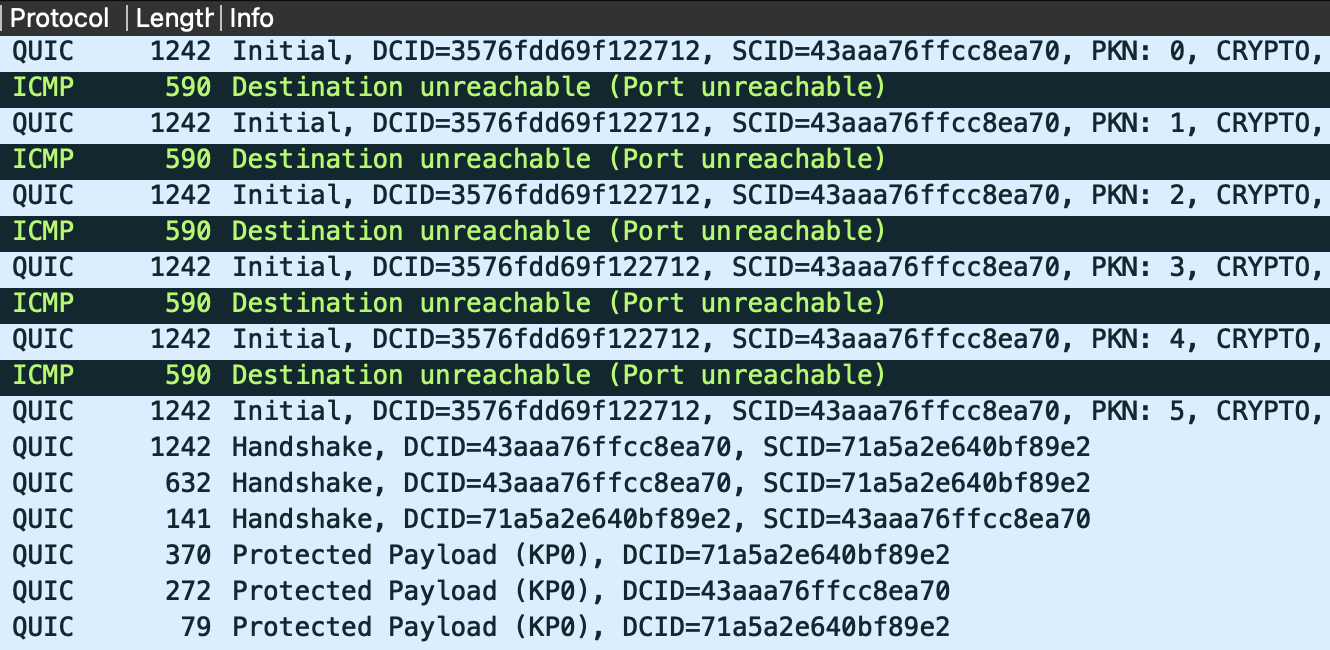
\includegraphics[width=\linewidth]{figs/quic-eva.png}
  \caption{手法2の実行結果}
  \label{fig:eva-2}
\end{figure}

手法2の通信確立が確認できた際のピア間のパケットキャプチャの様子を図~\ref{fig:eva-2}に示す.クライアント側が接続を開始しても,サーバー側のNATマッピングがなされていない最初の数回の試行はDestination unreachableで失敗している.その後NAT越えが成功し,通信が確立している.

手法2が完全に実装できた際の評価などは次章で述べる.
